% Set \REVIEW to 1 to flatten all slide-by-slide reveals (each frame becomes
% a single page with all content visible). Set to 0 for the normal stepwise
% presentation.
\def\REVIEW{0}
\ifnum\REVIEW=1 \PassOptionsToClass{handout}{beamer}\fi

\documentclass[xcolor={dvipsnames},t]{beamer}

% Style/color themes
\usetheme{Malmoe}
\usecolortheme{spruce}
\usefonttheme[onlymath]{serif}
\setbeamercolor{item}{fg=PineGreen}

% Bullet-point styling
\setbeamertemplate{itemize item}[square]
\setbeamertemplate{itemize subitem}[triangle]
\setbeamertemplate{itemize subsubitem}[square]
\setbeamertemplate{itemize/enumerate subbody begin}{\vspace{0.5em}}

% Remove navigation symbols
\beamertemplatenavigationsymbolsempty

% Custom footer
\setbeamertemplate{footline}
{
  \leavevmode%
  \hbox{%
    \begin{beamercolorbox}[wd=.3\paperwidth,ht=2.25ex,dp=1ex,center]{author in head/foot}%
        \usebeamerfont{author in head/foot} Interdisciplinary Journal Club
    \end{beamercolorbox}%
    \begin{beamercolorbox}[wd=.7\paperwidth,ht=2.25ex,dp=1ex,center]{date in head/foot}%
        \usebeamerfont{date in head/foot}\insertshorttitle\hspace*{2ex}
        (\insertframenumber{} / \inserttotalframenumber)
    \end{beamercolorbox}
  }%
  \vskip0pt%
}

\usepackage{natbib}
\usepackage{amsmath,amsthm,amssymb}
\usepackage{mathtools}
\usepackage{mathrsfs}
\usepackage{physics}
\usepackage{bm}
\usepackage{bbm}
\usepackage{graphicx}
\usepackage{caption}
\usepackage{tikz}
\usepackage{appendixnumberbeamer} % backup slides are not counted in the footer total

\usetikzlibrary{arrows.meta, patterns, positioning}

% visible on=<2->: draw a TikZ scope only from that overlay on, keeping its space
\tikzset{
    invisible/.style={opacity=0},
    visible on/.style={alt={#1{}{invisible}}},
    alt/.code args={<#1>#2#3}{\alt<#1>{\pgfkeysalso{#2}}{\pgfkeysalso{#3}}},
}

\captionsetup[figure]{labelformat=empty}
% ./figures holds slide versions (scripts/slide_figures.py); the rest come from the notes, used in place
\graphicspath{ {./images/} {./figures/} {../fpe-examples/figures/} }

\let\olditemize=\itemize
\let\endolditemize=\enditemize
\renewenvironment{itemize}{\olditemize \itemsep=.5em }{\endolditemize}

\setbeamertemplate{institute}{}

% Notation (Gardiner's, with B = D for constant noise)
\newcommand{\gv}{\,|\,}
\newcommand{\Lop}{\mathcal{L}}
\newcommand{\cU}{\mathcal{U}}

% Interactive companions: run `npm run dev` in ../plot-lab and ../sde-explorer
% (ports 5174 and 5173), or point these at a deployed copy.
\newcommand{\plotlab}{http://localhost:5174/}
\newcommand{\sdeexplorer}{http://localhost:5173/}
% \demolinks{plot-lab query}{sde-explorer query}: buttons at the top right of a frame; either may be empty
\newcommand{\demolinks}[2]{%
    \begin{tikzpicture}[remember picture,overlay]
        \node[anchor=north east,inner sep=0pt] at ([xshift=-3mm,yshift=-10.3mm]current page.north east) {\scriptsize
            \if\relax\detokenize{#1}\relax\else\href{\plotlab?#1}{\beamergotobutton{Plot Lab}}\fi
            \if\relax\detokenize{#2}\relax\else\ \href{\sdeexplorer?#2}{\beamergotobutton{SDE Explorer}}\fi};
    \end{tikzpicture}%
}

% Equation numbers in the comments are Gardiner, Handbook of Stochastic Methods, 2nd ed.;
% the 4th edition renumbers them.

\title[The Fokker--Planck Equation]{The Fokker--Planck Equation \\ {\small Gardiner, \textit{Stochastic Methods}, Chapter 5}}
\author{Sean Ericson \\ {\small Interdisciplinary Journal Club}}
\date{October 28, 2026}
\titlegraphic{
\includegraphics[scale=0.14]{UO_Seal.png}}

\begin{document}
\frame{\titlepage}

\begin{frame}{Outline}
    \begin{enumerate}
        \item The Fokker--Planck equation: where it comes from
        \item The probability current
        \item Boundary conditions and topology
        \item Eigenfunction methods
        \item Stationary and quasi-stationary states
        \item First passage
        \item Examples
    \end{enumerate}
\end{frame}

% =========================================================
% 1. The Fokker-Planck equation
% =========================================================
\begin{frame}{The Differential Chapman--Kolmogorov Equation}
    \alert{Drift, diffusion, and jumps}
    \begin{itemize}
        \item<2-> For a Markov process, expanding Chapman--Kolmogorov over a short time step gives (summing over repeated indices)
        \begin{align*}
            \partial_t p(\bm z,t) = &\underbrace{-\partial_i\bigl[A^i(\bm z)\,p(\bm z,t)\bigr]}_{\text{drift}}
            + \underbrace{\tfrac12\,\partial_i\partial_j\bigl[B^{ij}(\bm z)\,p(\bm z,t)\bigr]}_{\text{diffusion}} \\
            &+ \underbrace{\int\dd\bm x\,\bigl[W(\bm z\gv\bm x)\,p(\bm x,t) - W(\bm x\gv\bm z)\,p(\bm z,t)\bigr]}_{\text{jumps: gain $-$ loss}}
        \end{align*}
        % G2 (3.4.22)
        \vspace{-1.5em}
        \item<3-> $A^i$: mean velocity; $B^{ij}$: growth rate of the covariance of small moves; $W$: rate of jumps
        \item<4-> Special cases: $A=B=0$, the \textit{master equation}; $B=W=0$, the \textit{Liouville equation}; $W=0$, the \textit{Fokker--Planck equation}
        \item<5-> $W=0$ $\iff$ continuous sample paths: the FPE describes continuous Markov processes
    \end{itemize}
\end{frame}

\begin{frame}{The Fokker--Planck Equation}
    \alert{The FPE in one dimension}
    \begin{itemize}
        \item<2-> In one dimension
        \[ \boxed{\;\partial_t p(x,t) = -\partial_x\bigl[A(x,t)\,p(x,t)\bigr] + \tfrac12\,\partial_x^2\bigl[B(x,t)\,p(x,t)\bigr]\;} \]
        % G2 (5.2.1)
        \vspace{-1.5em}
        \begin{itemize}
            \item<3-> A second-order parabolic partial differential equation
        \end{itemize}
        \item<4-> $A$: drift; $B\ge0$: diffusion coefficient
        \item<5-> Holds for the transition density $p(x,t\gv x_0,t_0)$, with $p(x,t_0\gv x_0,t_0)=\delta(x-x_0)$
        \item<6-> Linear, so it also holds for any one-time density,
        \[ p(x,t)=\int\dd x_0\,p(x,t\gv x_0,t_0)\,p(x_0,t_0) \]
        \item<7-> Also called the forward Kolmogorov (or Smoluchowski) equation
    \end{itemize}
\end{frame}

\begin{frame}{The Fokker--Planck Equation}
    \alert{The backward equation}
    \begin{itemize}
        \item<2-> The transition density $p(x,t\gv y,t')$ also obeys an equation in its \textit{initial} point $(y,t')$:
        \[ -\partial_{t'}\,p(x,t\gv y,t') = A(y,t')\,\partial_yp + \tfrac12B(y,t')\,\partial_y^2p \]
        % G2 (3.6.4)
        \item<3-> Derivation: split Chapman--Kolmogorov at $t'+\Delta t$, and expand in the moments of the short first step
        \item<4-> Expectation values, as functions of the initial point, obey the same equation:
        \[ u(y,t') = \bigl\langle f(x(t))\bigr\rangle_{x(t')=y} = \int\dd x\,f(x)\,p(x,t\gv y,t') \]
        \vspace{-1.5em}
        \item<5-> Forward: fix the start, evolve the end. Backward: fix the end, vary the start
        \item<6-> Natural for questions about the start: survival, exit times and splitting probabilities are all such averages
    \end{itemize}
\end{frame}

% Question: what's up with the stratonovich eq? Does that relate to FPE on a general manifold?
\begin{frame}{The Corresponding SDE}
    \alert{Two descriptions of one process}
    \begin{itemize}
        \item<2-> The FPE is equivalent to the It\^o stochastic differential equation
        \[ \dd x(t) = A(x,t)\,\dd t + \sqrt{B(x,t)}\;\dd W(t) \]
        \item<3-> Over a short $\Delta t$,
        \[ \langle\Delta x\rangle = A\,\Delta t,\qquad \langle(\Delta x)^2\rangle = B\,\Delta t + O(\Delta t^2) \]
        \item<4-> SDE describes individual sample paths. FPE describes evolution of the density of the ensemble
        \item<5-> Conventions to watch
        \begin{itemize}
            \item<6-> Stratonovich $\dd x=a\,\dd t+\sqrt B\circ\dd W$ has FPE drift $A=a+\tfrac14\partial_xB$
            \item<7-> With $B=D$: $\langle(\Delta x)^2\rangle=Dt$. Many texts write $\partial_tp=D'\partial_x^2p$, with $D'=D/2$
        \end{itemize}
    \end{itemize}
\end{frame}

\begin{frame}{A General Physical Model}
    \alert{Damped Brownian particle with inertia}
    \begin{itemize}
        \item<2-> Particle of mass $m$ in a potential $\cU(x)$, with friction $\gamma$, in a heat bath at temperature $T$ (Langevin):
        \begin{align*}
            \dd x &= v\,\dd t \\
            m\,\dd v &= -\gamma v\,\dd t - \cU'(x)\,\dd t + \sqrt{2\gamma k_BT}\;\dd W
        \end{align*}
        % G2 (5.3.90)-(5.3.91); Gardiner's beta is gamma here
        \item<3-> The stationary solution is Maxwell--Boltzmann,
        \[ p_s(x,v)\propto e^{-E/k_BT}; \quad E = \frac{1}{2}mv^2+\cU(x) \]
        \item<4-> The FPE for $p(x,v,t)$ is \textit{Kramers' equation}, in two variables
        \item<5-> Two time scales
        \begin{itemize}
            \item<6-> $\tau_v=m/\gamma$: friction damps the velocity to the local terminal velocity $-\cU'/\gamma$
            \item<7-> $\tau_x=\gamma/|\cU''|$: the position slides down a well of curvature $\cU''$
        \end{itemize}
    \end{itemize}
\end{frame}

% Question: why is this limit equvalent to m \dd v = 0?
\begin{frame}{A General Physical Model}
    \alert{The overdamped limit}
    \begin{itemize}
        \item<2-> Overdamped: the velocity relaxes much faster than the position,
        \[ \varepsilon\equiv\frac{\tau_v}{\tau_x}=\frac{m|\cU''|}{\gamma^2}\ll1\quad\text{wherever the particle goes} \]
        \vspace{-1.5em}
        \begin{itemize}
            \item<3-> Harmonic trap $\cU=\tfrac12\mathcal Kx^2$: $\varepsilon=m\mathcal K/\gamma^2$
        \end{itemize}
        \item<4-> Over a step $\tau_v\ll\Delta t\ll\tau_x$, $m\,\Delta v$ stays bounded while the friction, force and noise impulses grow with $\Delta t$
        \begin{itemize}
            \item<5-> So $m\,\Delta v$ is negligible: friction balances force plus noise. Set $m\,\dd v\approx0$:
            \[ \gamma\,\dd x = -\cU'(x)\,\dd t + \sqrt{2\gamma k_BT}\;\dd W \]
        \end{itemize}
        \vspace{-1.5em}
        \item<6-> Valid for $t\gg\tau_v$, with corrections of order $\varepsilon$
    \end{itemize}
\end{frame}

% Question: is Smoluchowski's equation referenced in Gardiner?
% Question: what's the Einstein relation?
\begin{frame}{A General Physical Model}
    \alert{Smoluchowski's equation}
    \begin{itemize}
        \item<2-> An It\^o SDE with $A=-\cU'/\gamma$ and $B=D=2k_BT/\gamma$. Its FPE is Smoluchowski's equation
        \[ \partial_tp = \partial_x\Bigl[\frac{\cU'}{\gamma}\,p\Bigr] + \frac{k_BT}{\gamma}\,\partial_x^2p \]
        \vspace{-1.5em}
        \begin{itemize}
            \item<3-> $D/2 = k_BT/\gamma$ is the Einstein relation: diffusion $=$ temperature $\times$ mobility
            \item<4-> Writing $U=\cU/\gamma$: $A=-U'$, and $e^{-2U/D}=e^{-\cU/k_BT}$ is the Boltzmann factor
        \end{itemize}
        \item<5-> Done systematically, this is \textit{adiabatic elimination} of the fast variable $v$ (later in Gardiner)
        \begin{itemize}
            \item<6-> The first correction multiplies the diffusion by $1+m\cU''/\gamma^2=1\pm\varepsilon$
        \end{itemize}
    \end{itemize}
\end{frame}

% =========================================================
% 2. Probability current
% =========================================================
\begin{frame}{Probability Current}
    \alert{Definition and local conservation}
    \begin{itemize}
        \item<2-> In arbitrary dimensions:
        \[ \partial_tp = -\partial_i\bigl(A^i\,p\bigr) + \tfrac12\,\partial_i\partial_j\bigl(B^{ij}\,p\bigr) \]
        \item<3-> This is a continuity equation,
        \[ \partial_tp + \partial_iJ^i = 0,\qquad J^i = A^i\,p - \tfrac12\,\partial_j\bigl(B^{ij}\,p\bigr) \]
        % G2 (5.2.6)-(5.2.8)
        \item<4-> For a region $R$ with surface $S$, let $P(R,t)=\int_R\dd\bm z\,p(\bm z,t)$. Then
        \[ \partial_tP(R,t) = -\oint_S\dd S\;\hat n_i\,J^i(\bm z,t) \]
        % G2 (5.2.9)
        \item<5-> Probability leaves $R$ only through its surface, like charge
    \end{itemize}
\end{frame}

% Question: explain how the continuity equation alone fixes J only up to a divergence-free field.
\begin{frame}{Probability Current}
    \alert{Flux across any surface}
    \begin{columns}[T]
        \begin{column}{0.4\textwidth}
            \centering
            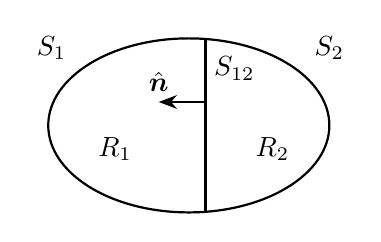
\begin{tikzpicture}[scale=0.85]
                \draw[thick] (0,0) ellipse (2.1 and 1.3);
                \draw[thick] (0.25,1.29) -- (0.25,-1.29);
                \node at (-1.1,-0.35) {$R_1$};
                \node at (1.25,-0.35) {$R_2$};
                \draw[-{Stealth},thick] (0.25,0.35) -- (-0.45,0.35) node[above] {$\hat{\bm n}$};
                \node at (-2.05,1.15) {$S_1$};
                \node at (2.1,1.15) {$S_2$};
                \node at (0.68,0.85) {$S_{12}$};
            \end{tikzpicture}
        \end{column}
        \begin{column}{0.6\textwidth}
            \begin{itemize}
                \item<2-> Stronger: $\bm J$ gives the net flow across \textit{any} surface, not just a closed one
                \item<3-> Net flow from $R_2$ to $R_1$ per unit time:
            \end{itemize}
        \end{column}
    \end{columns}
    \onslide<3->{
        {\footnotesize
        \[ \lim_{\Delta t\to0}\frac{1}{\Delta t}\int_{R_1}\!\dd\bm x\int_{R_2}\!\dd\bm y\,\bigl[p(\bm x,t+\Delta t;\bm y,t)-p(\bm y,t+\Delta t;\bm x,t)\bigr] = \int_{S_{12}}\!\dd S\;\hat n_iJ^i \]}
        % G2 (5.2.12), Fig. 5.1
    }
    \vspace{-1em}
    \begin{itemize}
        \item<4-> Why: paths are continuous, so in a short $\Delta t$ only particles near $S_{12}$ cross it. Use the FPE and the divergence theorem; the integrals over $S_1$ and $S_2$ vanish
        \item<5-> The continuity equation alone fixes $\bm J$ only up to a divergence-free field; this shows that the $\bm J$ above is the physical flux
    \end{itemize}
\end{frame}

\begin{frame}{Probability Current}
    \alert{One dimension: normalisation and boundaries}
    \begin{itemize}
        \item<2-> In one dimension $\partial_tp = -\partial_xJ$, so on $(a,b)$
        \[ \dv{t}\int_a^b p\,\dd x = J(a,t) - J(b,t) \]
        \item<3-> Boundary conditions are statements about the current at the ends
        \begin{itemize}
            \item<4-> $J=0$ at both ends: normalisation is conserved
            \item<5-> $J(b)=J(a)$: what leaves at one end comes back at the other (a circle; reinjection at $\pm\infty$)
            \item<6-> Outflow allowed: $\int p\,\dd x$ decreases. It is the probability of not yet having left
        \end{itemize}
        \item<7-> Stationary: $\partial_tp=0\implies\partial_xJ=0\implies J=\text{const}$
        % G2 (5.2.35)-(5.2.37)
        \begin{itemize}
            \item<8-> Either zero everywhere, or a steady current around a loop
        \end{itemize}
    \end{itemize}
\end{frame}

% =========================================================
% 3. Boundary conditions and topology
% =========================================================
\begin{frame}{Boundary Conditions}
    \alert{Four domains in one dimension}
    \begin{center}
        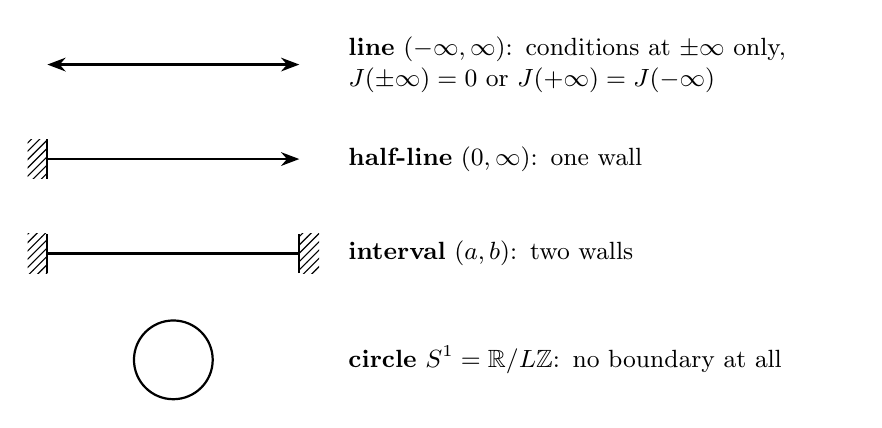
\begin{tikzpicture}[x=1cm,y=1cm, every node/.style={font=\small}]
            \begin{scope}[visible on=<2->]
                \draw[{Stealth}-{Stealth},thick] (0,3.6) -- (3.2,3.6);
                \node[anchor=west,text width=6.3cm] at (3.7,3.6) {\textbf{line} $(-\infty,\infty)$: conditions at $\pm\infty$ only, $J(\pm\infty)=0$ or $J(+\infty)=J(-\infty)$};
            \end{scope}
            \begin{scope}[visible on=<3->]
                \fill[pattern=north east lines] (-0.25,2.15) rectangle (0,2.65);
                \draw[thick] (0,2.15) -- (0,2.65);
                \draw[-{Stealth},thick] (0,2.4) -- (3.2,2.4);
                \node[anchor=west,text width=6.3cm] at (3.7,2.4) {\textbf{half-line} $(0,\infty)$: one wall};
            \end{scope}
            \begin{scope}[visible on=<4->]
                \fill[pattern=north east lines] (-0.25,0.95) rectangle (0,1.45);
                \fill[pattern=north east lines] (3.2,0.95) rectangle (3.45,1.45);
                \draw[thick] (0,0.95) -- (0,1.45);
                \draw[thick] (3.2,0.95) -- (3.2,1.45);
                \draw[thick] (0,1.2) -- (3.2,1.2);
                \node[anchor=west,text width=6.3cm] at (3.7,1.2) {\textbf{interval} $(a,b)$: two walls};
            \end{scope}
            \begin{scope}[visible on=<5->]
                \draw[thick] (1.6,-0.15) circle (0.5);
                \node[anchor=west,text width=6.3cm] at (3.7,-0.15) {\textbf{circle} $S^1=\mathbb R/L\mathbb Z$: no boundary at all};
            \end{scope}
        \end{tikzpicture}
    \end{center}
    \begin{itemize}
        \item<6-> Boundary conditions are part of the definition of the problem
        \item<7-> The same differential operator with different walls is a different operator, with a different spectrum
    \end{itemize}
\end{frame}

\begin{frame}{Boundary Conditions}
    \alert{Reflecting and absorbing walls}
    \begin{itemize}
        \item<2-> \textbf{Reflecting}: no net flow across the boundary $S$
        \[ \hat n_i\,J^i = 0 \ \text{ on } S \qquad (\text{1D}, A=0, B=D\text{: } \partial_xp=0,\ \text{Neumann}) \]
        % G2 (5.2.13)
        \vspace{-1.5em}
        \begin{itemize}
            \item<3-> A hard wall, $\cU\to\infty$
        \end{itemize}
        \item<4-> \textbf{Absorbing}: the particle is removed the moment it reaches $S$
        \[ p = 0\ \text{ on } S \qquad (\text{Dirichlet}) \]
        % G2 (5.2.14)
        \vspace{-1.5em}
        \begin{itemize}
            \item<5-> A cliff, a detector, a firing threshold, extinction, etc.
        \end{itemize}
        \item<6-> At an interface where $A$ or $B$ jumps: $\hat n_i\,J^i$ and $p$ are continuous
        % G2 (5.2.15)-(5.2.16)
    \end{itemize}
\end{frame}

\begin{frame}{Boundary Conditions}
    \alert{Reflecting, absorbing, and periodic}
    %\demolinks{page=physical}{}
    \vspace{-0.5em}
    \begin{center}
        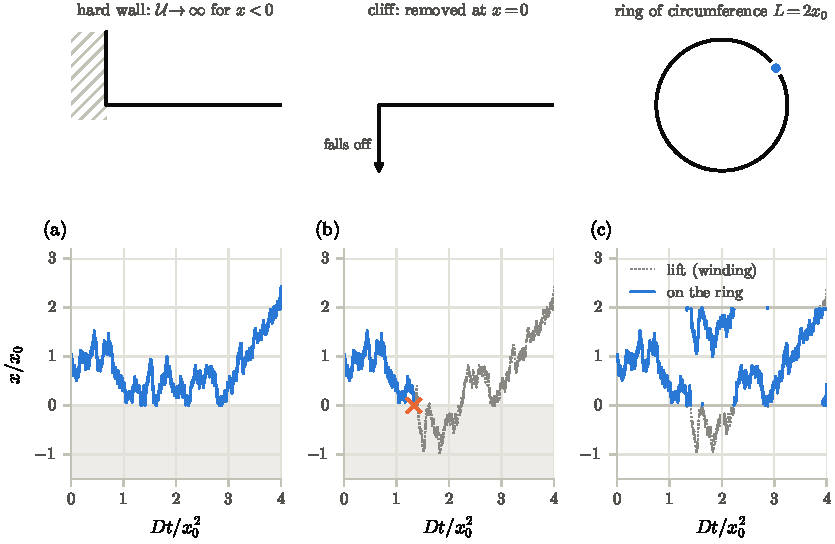
\includegraphics[width=0.96\textwidth]{walls_slides.pdf}
    \end{center}
\end{frame}

% Question: I need to know more about the "winding" thing before I can talk about it. I need a quick overview.
\begin{frame}{Boundary Conditions}
    \alert{Periodic boundaries, or: the circle}
    \begin{itemize}
        \item<2-> Gardiner: an interval $[a,b]$ with its ends identified, imposing (as at a discontinuity)
        \[ p(b^-,t)=p(a^+,t),\qquad J(b^-,t)=J(a^+,t) \]
        % G2 (5.2.17)-(5.2.19)
        \vspace{-1.5em}
        \item<3-> Cleaner: the state space \textit{is} the circle $S^1=\mathbb R/L\mathbb Z$
        \begin{itemize}
            \item<4-> No boundary $\implies$ no boundary conditions
            \item<5-> $A$, $B$, $p$ are $L$-periodic; conservation is topological:
            \[ \dv{t}\oint p\,\dd x=-\oint\partial_xJ\,\dd x=0 \]
        \end{itemize}
        \vspace{-1em}
        \item<6-> New physics
        \begin{itemize}
            \item<7-> A steady current $J_s\neq0$ exists iff $\Phi=\oint 2A/B\,\dd x\neq0$ (e.g.\ a constant torque): a non-equilibrium steady state
            \item<8-> A new observable, the winding: the net distance traveled around
        \end{itemize}
    \end{itemize}
\end{frame}

\begin{frame}{Feller's Classification}
    \alert{When the equation decides}
    \begin{itemize}
        \item<2-> So far, walls at finite points where $B>0$ and $A$ is bounded: we choose the condition
        \item<3-> Where $B\to0$ or $A\to\infty$, the equation itself may allow or forbid a condition
        \item<4-> Gardiner's quick rule: motion in $x>a$, with $B(a)=0$ and a Lipschitz condition,
        % G2 (5.2.20)-(5.2.24)
        \begin{itemize}
            \item<5-> $A(a)<0$: \textbf{exit}. A particle that reaches $a$ leaves the region
            \item<6-> $A(a)>0$: \textbf{entrance}. A particle at $a$ is pushed back in; particles can be introduced there
            \item<7-> $A(a)=0$: \textbf{natural}. Can be neither reached nor left
        \end{itemize}
        \item<8-> In general (Feller) there are four types: these three, plus \textbf{regular}, which is where we choose
    \end{itemize}
\end{frame}

\begin{frame}{Feller's Classification}
    \alert{The general test}
    \begin{itemize}
        \item<2-> With $x_0$ inside the domain, define
        % G2 (5.2.25)-(5.2.28)
        \begin{gather*}
            f(x)=\exp\Bigl[-2\!\int_{x_0}^x\!\frac{A}{B}\,\dd s\Bigr],\qquad g(x)=\frac{2}{B(x)\,f(x)}, \\
            h_1(x)=f(x)\!\int_{x_0}^x\!g\,\dd s,\qquad h_2(x)=g(x)\!\int_{x_0}^x\!f\,\dd s
        \end{gather*}
        \vspace{-1.5em}
        \item<3-> Integrability on $(a,x_0)$ decides the type of the boundary $a$:
    \end{itemize}
    \onslide<3->{
        \begin{table}
            \renewcommand{\arraystretch}{1.25}
            \resizebox{\textwidth}{!}{%
            \begin{tabular}{l|l|cc|l}
                \hline\hline
                Type & On $(a,x_0)$ & Reached? & Left? & Condition at $a$ \\
                \hline
                Regular  & $f$, $g$ integrable                  & yes & yes & must be chosen \\
                Exit     & $g$ not integrable, $h_1$ integrable & yes & no  & none (absorbs) \\
                Entrance & $g$ integrable, $h_2$ integrable     & no  & yes & none \\
                Natural  & all other cases                      & no  & no  & none \\
                \hline\hline
            \end{tabular}%
            }
        \end{table}
    }
    \begin{itemize}
        \item<4-> Exit: reached in finite mean time; no normalisable $p_s$. Entrance: $p_s$ can exist; never reached
        % G2 p.123: the second "exit" in the paragraph after (5.2.29) should read "entrance"
    \end{itemize}
\end{frame}

% Question: I like this example but I don't understand it enough. Give me an explanation of each graph (particularly the second and third ones, but also what the x is in the first)
\begin{frame}{Feller's Classification}
    \alert{Example: the squared radius}
    \demolinks{page=sqrt}{}
    \begin{center}
        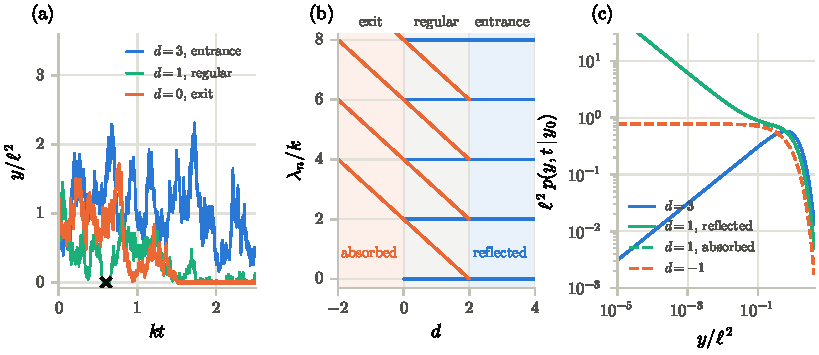
\includegraphics[width=0.92\textwidth]{sqrt.pdf}
    \end{center}
    \vspace{-1em}
    \begin{itemize}
        \small
        \item<2-> $y=r^2$ in a $d$-dimensional harmonic trap: $\dd y=(dD-2ky)\,\dd t+\sqrt{4Dy}\;\dd W$
        \item<3-> $d\ge2$: entrance (Brownian motion in $\ge2$ dimensions misses points); $0<d<2$: regular; $d\le0$: exit (extinction)
        \item<4-> The quick rule fails here ($\sqrt B$ not Lipschitz): $A(0)=dD>0$ for all $d>0$
    \end{itemize}
\end{frame}

% =========================================================
% 4. Eigenfunction methods
% =========================================================
\begin{frame}{It's Linear Algebra Time}
    \alert{The forward and backward operators}
    \begin{itemize}
        \item<2-> Homogeneous process: $p$ depends on $t-t'$ only, so take $t'=0$. Forward (Fokker--Planck) operator, acting on the final point $x$:
        \[ \partial_t\,p(x,t\gv y,0)=\Lop_x\,p(x,t\gv y,0),\quad \Lop p = -\partial_x(Ap) + \tfrac12\,\partial_x^2(Bp) \]
        \item<3-> Backward operator, acting on the initial point $y$:
        \[ \partial_t\,p(x,t\gv y,0)=\Lop^\dagger_y\,p(x,t\gv y,0),\qquad \Lop^\dagger f = A\,\partial_yf + \tfrac12B\,\partial_y^2f \]
        \item<4-> Averages from a start at $y$, $u(y,t)=\int\dd x\,f(x)\,p(x,t\gv y,0)$, obey $\partial_tu=\Lop^\dagger_y\,u$
        \begin{itemize}
            \item<5-> $\Lop$ moves probability forward in time; $\Lop^\dagger$ (the \textit{generator}) moves observables
        \end{itemize}
    \end{itemize}
\end{frame}

% Question: on the last line, does that say that they're only adjoint when that last term is zero? When is that the case?
\begin{frame}{It's Linear Algebra Time}
    \alert{Adjoint operators}
    \begin{itemize}
        \item<2-> Densities $p$ ($\int|p|<\infty$: the space $L^1$) and bounded observables $f$ (the space $L^\infty$) are paired by the expectation value, $\langle f,p\rangle = \int_a^b f\,p\,\dd x$
        \item<3-> No inner product needed: $\Lop^\dagger$ is the adjoint of $\Lop$ if $\langle f,\Lop p\rangle=\langle\Lop^\dagger f,p\rangle$. Integrating by parts,
        \[ \langle f,\Lop p\rangle - \langle\Lop^\dagger f,p\rangle = \Bigl[-fJ - \tfrac12Bp\,\partial_xf\Bigr]_a^b \]
        \item<4-> An operator includes its domain (the boundary conditions). They are adjoint when this vanishes for every allowed $p$ and $f$:
        \begin{itemize}
            \item<5-> absorbing: $p=0$ forces $f=0$; \ reflecting: $J=0$ forces $\partial_xf=0$
            % G2 (5.2.65), (5.2.67), (5.2.69)
            \item<6-> circle: no boundary, nothing to check
        \end{itemize}
    \end{itemize}
\end{frame}

\begin{frame}{Eigenfunction Methods}
    \alert{Gardiner's $P_\lambda$ and $Q_\lambda$}
    \begin{itemize}
        \item<2-> Homogeneous process on $(a,b)$, reflecting walls, stationary solution $p_s$
        \item<3-> Substituting $p(x,t)=p_s(x)\,q(x,t)$ gives the backward equation for $q$:
        \[ \partial_tq = A\,\partial_xq + \tfrac12B\,\partial_x^2q \]
        % G2 (5.2.71)-(5.2.72); needs zero stationary current
        \item<4-> Separable solutions $p=P_\lambda(x)\,e^{-\lambda t}$ and $q=Q_\lambda(x)\,e^{-\lambda t}$:
        \[ \Lop P_\lambda=-\lambda P_\lambda,\qquad \Lop^\dagger Q_\lambda=-\lambda Q_\lambda,\qquad P_\lambda(x)=p_s(x)\,Q_\lambda(x) \]
        % G2 (5.2.73)-(5.2.76)
        \vspace{-1.5em}
        \begin{itemize}
            \item<5-> $P_\lambda$: a density profile that keeps its shape and decays at rate $\lambda$
            \item<6-> $Q_\lambda$: a function of the starting point; $Q_\lambda(x_0)$ is how strongly a start at $x_0$ excites mode $\lambda$
            \item<7-> $P_\lambda=p_sQ_\lambda$ needs zero stationary current; then one set gives the other
        \end{itemize}
    \end{itemize}
\end{frame}

% Question: What exactly is the space L^2 you mention? I think this will get cleared up when addressing my previous concerns about inner product spaces and stuff
\begin{frame}{Eigenfunction Methods}
    \alert{Biorthogonality}
    \begin{itemize}
        \item<2-> Integrating by parts (the boundary terms vanish with paired walls):
        \[ (\lambda'-\lambda)\int_a^b P_\lambda\,Q_{\lambda'}\,\dd x = 0 \]
        % G2 (5.2.77)-(5.2.78)
        \item<3-> So, normalised,
        \[ \int_a^b P_\lambda\,Q_{\lambda'}\,\dd x = \int_a^b p_s\,Q_\lambda\,Q_{\lambda'}\,\dd x = \int_a^b \frac{P_\lambda\,P_{\lambda'}}{p_s}\,\dd x = \delta_{\lambda\lambda'} \]
        % G2 (5.2.79)-(5.2.81)
        \item<4-> $\lambda=0$ is the stationary solution: $P_0=p_s$, $Q_0=1$
        % G2 (5.2.82)-(5.2.83)
        \item<5-> Why two sets? In $L^2(a,b)$, with $\langle f,g\rangle=\int fg\,\dd x$, $\Lop$ is not symmetric (unless $p_s$ is uniform)
        \begin{itemize}
            \item<6-> $P_\lambda$ are its right eigenvectors; $Q_\lambda$, the eigenvectors of $\Lop^\dagger$, its left ones
        \end{itemize}
        \item<7-> In $L^2(1/p_s)$, $\langle p,q\rangle=\int pq/p_s\,\dd x$: $\Lop$ \textit{is} symmetric, the $P_\lambda$ orthonormal
    \end{itemize}
\end{frame}

\begin{frame}{Eigenfunction Methods}
    \alert{Expanding any solution}
    \begin{itemize}
        \item<2-> Any solution is
        \[ p(x,t) = \sum_\lambda A_\lambda\,P_\lambda(x)\,e^{-\lambda t},\qquad A_\lambda=\int_a^b Q_\lambda(x)\,p(x,0)\,\dd x \]
        % G2 (5.2.84)-(5.2.85)
        \vspace{-1.5em}
        \item<3-> An initial condition $p(x,0) = \delta(x-x_0)$ has $A_\lambda=Q_\lambda(x_0)$, so
        \[ \boxed{\;p(x,t\gv x_0,0) = \sum_\lambda P_\lambda(x)\,Q_\lambda(x_0)\,e^{-\lambda t}\;} \]
        % G2 (5.2.88)
        \vspace{-1.5em}
        \item<4-> Stationary autocorrelation:
        \[ \langle x(t)x(0)\rangle_s = \sum_\lambda\Bigl[\int x\,P_\lambda(x)\,\dd x\Bigr]^2 e^{-\lambda t} \]
        % G2 (5.2.90)
        % G2 (5.2.91)
    \end{itemize}
\end{frame}

% Question: explain the propagator line
\begin{frame}{Analogy with Quantum Mechanics}
    \alert{Imaginary time}
    \onslide<2->{
        \begin{table}
            \renewcommand{\arraystretch}{1.35}
            \resizebox{\textwidth}{!}{%
            \begin{tabular}{r|c|c}
                \hline\hline
                & Quantum mechanics & Fokker--Planck \\
                \hline
                Equation         & $i\hbar\,\partial_t\psi = H\psi$                                & $\partial_tp=\Lop p$ \\
                Modes            & $H\phi_n = E_n\phi_n$                                           & $\Lop P_\lambda=-\lambda P_\lambda$, \ $\Lop^\dagger Q_\lambda=-\lambda Q_\lambda$ \\
                Time dependence  & $e^{-iE_nt/\hbar}$: a phase                                     & $e^{-\lambda t}$: decay \\
                General solution & $\sum_n c_n\,\phi_n\,e^{-iE_nt/\hbar}$                          & $\sum_\lambda A_\lambda\,P_\lambda\,e^{-\lambda t}$ \\
                Coefficients     & $c_n=\int\phi_n^*\,\psi(0)$                                     & $A_\lambda=\int Q_\lambda\,p(0)$ \\
                Propagator       & $\sum_n\phi_n(x)\,\phi_n^*(x_0)\,e^{-iE_nt/\hbar}$              & $\sum_\lambda P_\lambda(x)\,Q_\lambda(x_0)\,e^{-\lambda t}$ \\
                Lowest mode      & ground state                                                    & stationary state, $\lambda=0$ \\
                \hline\hline
            \end{tabular}%
            }
        \end{table}
    }
    \begin{itemize}
        \item<3-> Each mode's time evolution is trivial: all the work is in the time-independent eigenproblem
        \item<4-> Differences: $\lambda\ge0$ are decay rates; $p$ itself (not $|\psi|^2$) is the probability; $Q_\lambda\neq P_\lambda^*$
    \end{itemize}
\end{frame}

% =========================================================
% 5. Stationary and quasi-stationary states
% =========================================================
\begin{frame}{Stationary States}
    \alert{Zero current: the potential solution}
    \begin{itemize}
        \item<2-> $J$ is constant; with a reflecting wall anywhere, $J=0$ everywhere. Then $A\,p_s=\tfrac12\,\partial_x(B\,p_s)$, so
        \[ \boxed{\;p_s(x) = \frac{\mathcal N}{B(x)}\exp\Bigl[2\!\int^x\!\frac{A(x')}{B(x')}\,\dd x'\Bigr]\;} \]
        % G2 (5.2.38)-(5.2.39)
        \vspace{-1.5em}
        \item<3-> A stationary state exists iff this is normalisable
        \item<4-> Overdamped particle: $p_s\propto e^{-2U/D}=e^{-\cU/k_BT}$, the Boltzmann distribution
        \item<5-> Examples (constant $B(x) = D$):
        \begin{itemize}
            \item<6-> $A=0$: uniform on an interval; on the half-line not normalisable, so no stationary state
            \item<7-> $A=v$: barometric, $e^{2vx/D}$ (sedimentation)
            \item<8-> $A=-kx$: Gaussian $e^{-kx^2/D}$, with variance $D/2k$
        \end{itemize}
    \end{itemize}
\end{frame}

\begin{frame}{Stationary States}
    \alert{From the eigenfunction expansion}
    \begin{itemize}
        \item<2-> Separate the $\lambda=0$ term:
        \[ p(x,t\gv x_0,0) = p_s(x)\cdot1 + \sum_{\lambda>0}P_\lambda(x)\,Q_\lambda(x_0)\,e^{-\lambda t} \]
        \item<3-> Every other term decays, so $p\to p_s$ from every start
        \item<4-> The slowest, $\lambda_1$ (the \textit{spectral gap}), sets the approach:
        \[ p-p_s\simeq P_1(x)\,Q_1(x_0)\,e^{-\lambda_1t} \]
        \vspace{-1.5em}
        \begin{itemize}
            \item<5-> Relaxation time $1/\lambda_1$, for correlation functions too
            \item<6-> If $Q_1(x_0)=0$ (start at the centre of a symmetric box), the next mode dominates
        \end{itemize}
        \item<7-> Normalisation sits in $\lambda=0$ alone: $\int P_\lambda\,\dd x=\int P_\lambda\,Q_0\,\dd x=0$ for $\lambda\neq0$
        \begin{itemize}
            \item<8-> The other modes only move probability around, so each changes sign
        \end{itemize}
    \end{itemize}
\end{frame}

% Question: explain the last one to me. the lowest eigenvalue isn't zero?
\begin{frame}{The Spectral Gap}
    \alert{Example spectra}
    \demolinks{page=spectra}{}
    \begin{center}
        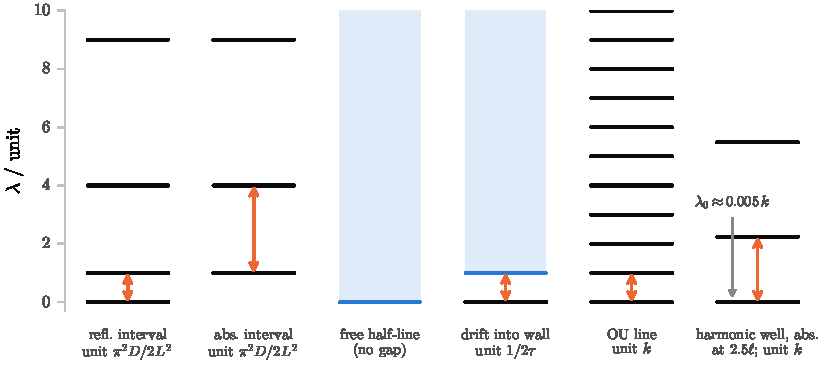
\includegraphics[width=\textwidth]{spectra.pdf}
    \end{center}
\end{frame}

% Question: briefly explain why it's the difference \lambda_2 - \lambda_1 that sets the rate of approach to QSD
\begin{frame}{Quasi-Stationary Distributions}
    \alert{Absorbing walls}
    \begin{itemize}
        \item<2-> No $\lambda=0$ mode: every mode decays, and $p\to0$
        \item<3-> Survival probability
        \[ S(t)=\int p\,\dd x \simeq Q_1(x_0)\Bigl[\int P_1\,\dd x\Bigr]e^{-\lambda_1t} \]
        \item<4-> Conditioned density $\tilde p=p/S\to P_1/\!\int P_1\,\dd x$: the \textit{quasi-stationary distribution} (QSD)
        \begin{itemize}
            \item<5-> The shape stops changing while the total probability decays
        \end{itemize}
        \item<6-> Two rates: $\lambda_1$ is the absorption rate; $\lambda_2-\lambda_1$ is the rate of approach to the QSD
        \item<7-> Metastability: if $\lambda_2-\lambda_1\gg\lambda_1$, the particle equilibrates locally long before it escapes, and escape is Poisson at rate $\lambda_1$
    \end{itemize}
\end{frame}

\begin{frame}{Quasi-Stationary Distributions}
    \alert{Example: free diffusion between two cliffs}
    \demolinks{page=interval}{a=0&b=sqrt(D)&p=D:1&lo=0&hi=1&bc=absorbing,absorbing&x0=0.3&T=0.5&cond=1}
    \begin{center}
        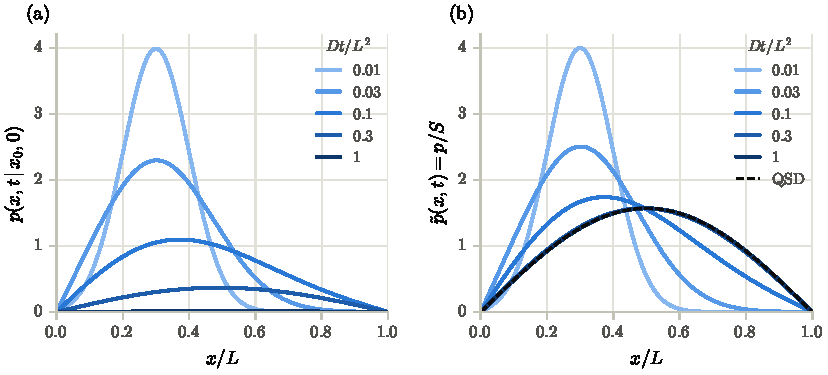
\includegraphics[width=0.85\textwidth]{absorbing_density_slides.pdf}
    \end{center}
    \vspace{-1.5em}
    \begin{itemize}
        \small
        \item<2-> $A=0$, $B=D$ on $(0,L)$, absorbing: $Q_n=\sqrt2\sin(n\pi x/L)$, $P_n=Q_n/L$, $\lambda_n=n^2\pi^2D/2L^2$
        \item<3-> (a) The density shrinks; (b) $\tilde p=p/S$ settles on the QSD $\tfrac{\pi}{2L}\sin(\pi x/L)$, at rate $\lambda_2-\lambda_1=3\lambda_1$
    \end{itemize}
\end{frame}

\begin{frame}{Quasi-Stationary Distributions}
    \alert{A caution about unbounded domains}
    \begin{itemize}
        \item<2-> Bounded domain: exactly one QSD, and every start reaches it
        \item<3-> Unbounded: there may be none, or a continuum
        \begin{itemize}
            \item<4-> Free half-line, absorbing at $0$: none ($S\sim t^{-1/2}$)
            \item<5-> Drift toward an absorbing wall: one for every $\lambda\in(0,v^2/2D]$
            \item<6-> OU absorbed at the bottom of its well: one for every $\lambda\in(0,k]$
        \end{itemize}
        \item<7-> With a continuum, the initial distribution selects the $\lambda$ that dominates at long times
        \item<8-> Unique, attracting QSD iff $\infty$ is an \textit{entrance} boundary: the mean absorption time stays bounded as $x_0\to\infty$
    \end{itemize}
\end{frame}

% =========================================================
% 6. First passage
% =========================================================
\begin{frame}{First Passage}
    \alert{Survival probability}
    \begin{itemize}
        \item<2-> Absorbing walls at $a$ and $b$, start at $x_0\in(a,b)$, exit time $T$:
        \[ G(x_0,t) = \int_a^b p(x,t\gv x_0,0)\,\dd x = \text{Prob}(T>t) \]
        % G2 (5.2.140)
        \vspace{-1.5em}
        \item<3-> Integrating the backward equation over $x$:
        \[ \partial_tG = A(x_0)\,\partial_{x_0}G + \tfrac12B(x_0)\,\partial_{x_0}^2G \]
        with $G(x_0,0)=1$ and $G(a,t)=G(b,t)=0$ (a reflecting end has $\partial_{x_0}G=0$)
        % G2 (5.2.144)-(5.2.146)
        \item<4-> Exit-time density $-\partial_tG$: the current out through the walls, $-J(a,t)+J(b,t)$
        \item<5-> From the expansion: $G(x_0,t)=\sum_\lambda Q_\lambda(x_0)\,e^{-\lambda t}\int P_\lambda\,\dd x\;\sim\;e^{-\lambda_1t}$
    \end{itemize}
\end{frame}

\begin{frame}{First Passage}
    \alert{Example: free diffusion between two cliffs}
    \begin{center}
        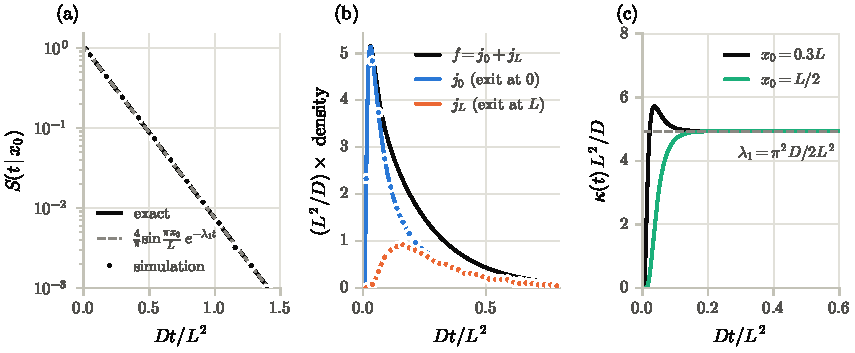
\includegraphics[width=\textwidth]{absorbing_exit.pdf}
    \end{center}
    \vspace{-1em}
    \begin{itemize}
        \small
        \item<2-> (a) Survival: exact, one-mode approximation, and simulation
        \item<3-> (b) Exit-time density, split into the currents out through each wall
        \item<4-> (c) Exit rate $-\dot S/S$ tends to $\lambda_1=\pi^2D/2L^2$ from every start
    \end{itemize}
\end{frame}

\begin{frame}{First Passage}
    \alert{Mean exit time}
    \begin{itemize}
        \item<2-> $T(x_0)=\langle T\rangle=\int_0^\infty G\,\dd t$. Integrating the backward equation over $t$ ($G$ goes from $1$ to $0$):
        \[ A(x_0)\,T'(x_0) + \tfrac12B(x_0)\,T''(x_0) = -1,\qquad T(a)=T(b)=0 \]
        % G2 (5.2.154)
        \vspace{-1.5em}
        \begin{itemize}
            \item<3-> Higher moments: $A\,T_n'+\tfrac12B\,T_n''=-n\,T_{n-1}$
            % G2 (5.2.156)
        \end{itemize}
        \item<4-> With $\psi(x)=\exp\int^x 2A/B\,\dd x'$, \ $I(x)=\int_a^x\frac{\dd y}{\psi(y)}$ \ and \ $F(x)=2\int_a^x\frac{\dd y}{\psi(y)}\int_a^y\frac{\psi(z)}{B(z)}\,\dd z$:
        \[ \boxed{\;T(x_0) = \frac{I(x_0)}{I(b)}\,F(b) - F(x_0)\;}\qquad\text{(both walls absorbing)} \]
        % G2 (5.2.157)-(5.2.158), rearranged
        \vspace{-1.5em}
        \begin{itemize}
            \item<5-> Reflecting at $a$ instead: $T(x_0)=F(b)-F(x_0)$
            % G2 (5.2.160)
        \end{itemize}
        \item<6-> Free diffusion, both walls absorbing: $T(x_0)=(x_0-a)(b-x_0)/D$
    \end{itemize}
\end{frame}

\begin{frame}{First Passage}
    \alert{Splitting probabilities}
    \begin{itemize}
        \item<2-> $\pi_a(x_0)$, $\pi_b(x_0)$: probability of leaving through $a$, or through $b$; $\pi_a+\pi_b=1$
        \item<3-> Same operator, no source:
        \[ A\,\pi_b' + \tfrac12B\,\pi_b'' = 0,\qquad \pi_b(a)=0,\quad \pi_b(b)=1 \]
        % G2 (5.2.186)-(5.2.187)
        \vspace{-1.5em}
        \item<4-> Solution, with $I$ from the last slide:
        \[ \pi_b(x_0) = \frac{I(x_0)}{I(b)} = \frac{\int_a^{x_0}\dd y/\psi(y)}{\int_a^b\dd y/\psi(y)} \]
        % G2 (5.2.189)-(5.2.190) print psi where 1/psi is correct
        \vspace{-1em}
        \item<5-> Free diffusion: $\pi_b=(x_0-a)/(b-a)$
        \item<6-> Constant drift $v$:
        \[ \pi_b=\frac{1-e^{-2v(x_0-a)/D}}{1-e^{-2v(b-a)/D}} \]
    \end{itemize}
\end{frame}

% =========================================================
% 7. Examples
% =========================================================
\begin{frame}{Examples}
    \alert{How the problems reduce to each other}
    \demolinks{page=reductions}{}
    \begin{center}
        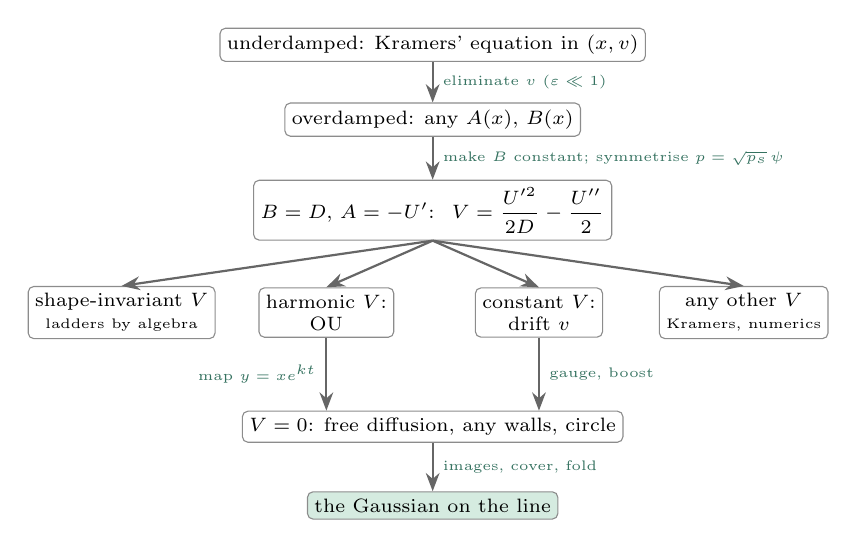
\begin{tikzpicture}[x=1cm,y=1cm,
                box/.style={draw=black!45, rounded corners=2pt, fill=white, align=center, font=\scriptsize, inner sep=2.5pt},
                lab/.style={font=\tiny, text=PineGreen!70!black, align=center},
                arr/.style={-{Stealth}, thick, black!60}]
            \node[box] (under) at (0,5.6) {underdamped: Kramers' equation in $(x,v)$};
            \node[box] (over)  at (0,4.65) {overdamped: any $A(x)$, $B(x)$};
            \node[box] (sym)   at (0,3.5) {$B=D$, $A=-U'$: \ $V=\dfrac{U'^2}{2D}-\dfrac{U''}{2}$};
            \node[box] (shape) at (-3.95,2.2) {shape-invariant $V$\\{\tiny ladders by algebra}};
            \node[box] (harm)  at (-1.35,2.2) {harmonic $V$:\\OU};
            \node[box] (const) at (1.35,2.2) {constant $V$:\\drift $v$};
            \node[box] (other) at (3.95,2.2) {any other $V$\\{\tiny Kramers, numerics}};
            \node[box] (free)  at (0,0.75) {$V=0$: free diffusion, any walls, circle};
            \node[box, fill=PineGreen!15] (gauss) at (0,-0.25) {the Gaussian on the line};
            \draw[arr] (under) -- node[lab, right] {eliminate $v$ ($\varepsilon\ll1$)} (over);
            \draw[arr] (over) -- node[lab, right] {make $B$ constant; symmetrise $p=\sqrt{p_s}\,\psi$} (sym);
            \draw[arr] (sym.south) -- (shape.north);
            \draw[arr] (sym.south) -- (harm.north);
            \draw[arr] (sym.south) -- (const.north);
            \draw[arr] (sym.south) -- (other.north);
            \draw[arr] (harm.south) -- node[lab, left] {map $y=xe^{kt}$} (harm.south |- free.north);
            \draw[arr] (const.south) -- node[lab, right] {gauge, boost} (const.south |- free.north);
            \draw[arr] (free) -- node[lab, right] {images, cover, fold} (gauss);
        \end{tikzpicture}
    \end{center}
\end{frame}

\begin{frame}{Example: Free Diffusion on an Interval}
    \alert{One operator, two kinds of wall}
    \begin{itemize}
        \item<2-> $A=0$, $B=D$ on $(0,L)$. Images: mirror the line's Gaussian $g$ in both walls, then the mirrors in each other:
        \[ p(x,t\gv x_0,0)=\sum_{m\in\mathbb Z}\bigl[g(x-x_0+2mL,t)\pm g(x+x_0+2mL,t)\bigr] \]
        \vspace{-1.5em}
        \item<3-> $+$ reflecting, $-$ absorbing. Summed as a Fourier series instead:
    \end{itemize}
    \onslide<3->{
        {\footnotesize
        \begin{center}
            \renewcommand{\arraystretch}{1.2}
            \begin{tabular}{l|c|c}
                \hline\hline
                & Reflecting & Absorbing \\
                \hline
                Modes      & $Q_n=\sqrt2\cos(n\pi x/L)$, \ $n\ge0$ & $Q_n=\sqrt2\sin(n\pi x/L)$, \ $n\ge1$ \\
                Rates      & \multicolumn{2}{c}{$\lambda_n=n^2\pi^2D/2L^2$} \\
                Long times & $p_s=1/L$ & QSD $\propto\sin(\pi x/L)$ \\
                Exit       & never & $\pi_L=x_0/L$, \ $T=x_0(L-x_0)/D$ \\
                \hline\hline
            \end{tabular}
        \end{center}}
    }
    \begin{itemize}
        \item<4-> Same rates for $n\ge1$; only the reflecting box has $\lambda_0=0$
        \item<5-> $x\to L-x$: the modes alternate even, odd; a start at $L/2$ excites only even ones
    \end{itemize}
\end{frame}

\begin{frame}{Example: Free Diffusion in a Box}
    \demolinks{page=reflecting}{a=0&b=sqrt(D)&p=D:1&lo=0&hi=1&bc=reflecting,reflecting&x0=0.3&T=1}
    \begin{center}
        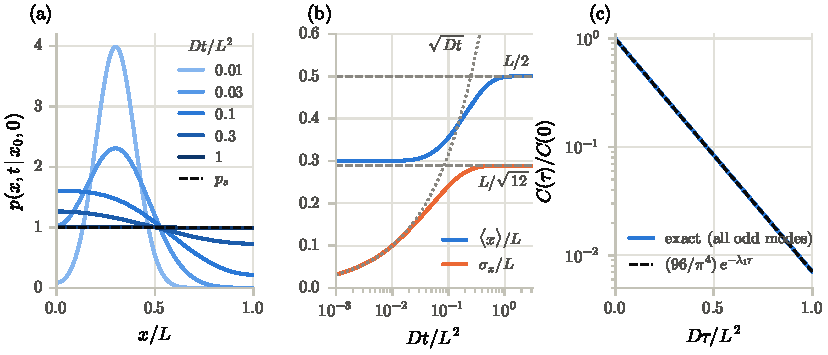
\includegraphics[width=\textwidth]{reflecting_slides.pdf}
    \end{center}
    \vspace{-1em}
    \begin{itemize}
        \small
        \item<2-> (a) From $x_0=0.3L$: a spreading Gaussian, then uniform
        \item<3-> (b) $\sigma_x$ grows like $\sqrt{Dt}$, then saturates at $L/\sqrt{12}$
        \item<4-> (c) $C(\tau)/C(0)\simeq(96/\pi^4)\,e^{-\lambda_1\tau}$: the gap dominates from the start
    \end{itemize}
\end{frame}

\begin{frame}{Example: Constant Drift on an Interval}
    \alert{Reduction to free diffusion}
    \begin{itemize}
        \item<2-> $A=v$, $B=D$ on $(0,L)$: sedimentation, an ion driven across a membrane. Scales $\ell=D/|v|$, $\tau=D/v^2$; one parameter, the P\'eclet number $vL/D=\pm L/\ell$
        \item<3-> Gauge: $p=e^{\alpha(x-x_0)-t/2\tau}\,u$ with $\alpha=v/D$, and $u$ diffuses freely
        \begin{itemize}
            \item<4-> $e^{\alpha x}\propto\sqrt{p_s}$: the symmetrisation, with constant $V=1/2\tau$. Rates are $u$'s plus $1/2\tau$
            \item<5-> Absorbing walls stay absorbing ($u=0$); reflecting ones become Robin ($\partial_xu=\alpha u$)
        \end{itemize}
    \end{itemize}
    \onslide<6->{
        {\footnotesize
        \begin{center}
            \renewcommand{\arraystretch}{1.25}
            \begin{tabular}{l|l|l}
                \hline\hline
                Walls at $0$, $L$ & Picture & Rates \\
                \hline
                reflecting, reflecting & closed column  & $0$; \ $1/2\tau+n^2\pi^2D/2L^2$, $n\ge1$ \\
                absorbing, absorbing   & two cliffs     & $1/2\tau+n^2\pi^2D/2L^2$, $n\ge1$ \\
                reflecting, absorbing  & floor and rim  & $1/2\tau+Dk^2/2$, \ $\tan kL=-k/\alpha$ \\
                \hline\hline
            \end{tabular}
        \end{center}}
    }
\end{frame}

\begin{frame}{Constant Drift: Reflecting Walls}
    \demolinks{page=drift-reflecting}{a=v&b=sqrt(D)&p=v:4,D:1&lo=0&hi=1&bc=reflecting,reflecting&x0=0.3&T=1}
    \begin{center}
        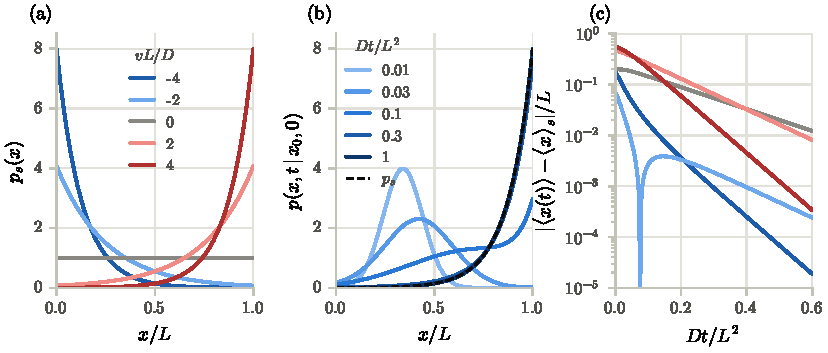
\includegraphics[width=0.95\textwidth]{drift_reflecting_slides.pdf}
    \end{center}
    \vspace{-1em}
    \begin{itemize}
        \small
        \item<2-> (a) $p_s\propto e^{2vx/D}$: barometric, piled against the downstream wall
        \item<3-> Robin at both ends keeps $k_n=n\pi/L$; the extra $\lambda_0=0$ is $u=e^{\alpha x}$
        \item<4-> (b) $vL/D=4$: carried downstream. (c) $\langle x\rangle$ relaxes at $\lambda_1$, the same for $\pm v$
    \end{itemize}
\end{frame}

\begin{frame}{Constant Drift: Absorbing Walls}
    \demolinks{page=drift-absorbing}{a=v&b=sqrt(D)&p=v:4,D:1&lo=0&hi=1&bc=absorbing,absorbing&x0=0.3&T=0.5&cond=1}
    \begin{center}
        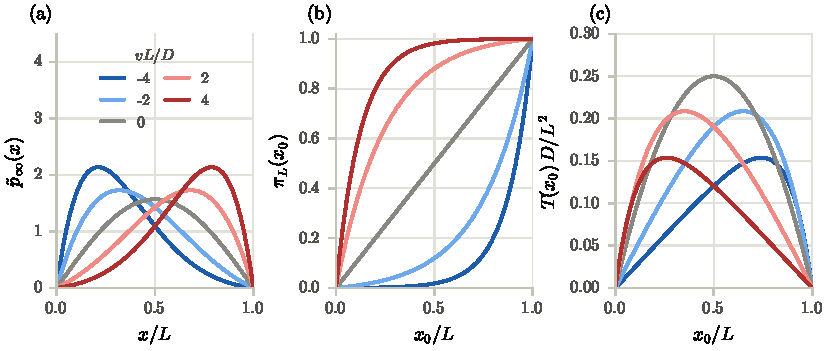
\includegraphics[width=0.9\textwidth]{drift_absorbing_slides.pdf}
    \end{center}
    \vspace{-1em}
    \begin{itemize}
        \small
        \item<2-> Tilted free sines: $P_n\propto e^{\alpha x}\sin k_nx$, $Q_n\propto e^{-\alpha x}\sin k_nx$, $k_n=n\pi/L$
        \item<3-> (a) QSD $\propto e^{\alpha x}\sin(\pi x/L)$, piled up downstream
        \item<4-> (b) Biased gambler's ruin, $\pi_L=(1-e^{-2\alpha x_0})/(1-e^{-2\alpha L})$
        \item<5-> (c) $T=(L\pi_L-x_0)/v$; strong drift gives the transit time $(L-x_0)/v$
        \item<6-> Mirror symmetry $x\to L-x$, $v\to-v$ pairs up the curves
    \end{itemize}
\end{frame}

\begin{frame}{Constant Drift: Escape over a Barrier}
    \demolinks{page=drift-mixed}{a=v&b=sqrt(D)&p=v:-2,D:1&lo=0&hi=1&bc=reflecting,absorbing&x0=0&T=20&cond=1}
    \begin{center}
        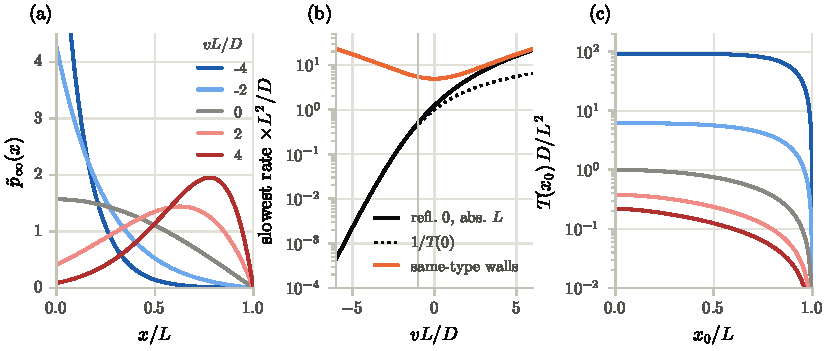
\includegraphics[width=0.88\textwidth]{drift_mixed_slides.pdf}
    \end{center}
    \vspace{-1em}
    \begin{itemize}
        \small
        \item<2-> Reflecting at $0$, absorbing at $L$: $\tan kL=-k/\alpha$
        \item<3-> $v<0$, $L>\ell$: $k$ turns imaginary: a bound state, rate below $1/2\tau$
        \item<4-> (b) Barrier $|v|L$: slowest rate $\simeq1/T\simeq(2/\tau)\,e^{-2L/\ell}$ (Arrhenius)
        \item<5-> (a) QSD $\to$ barometric, cut off at $L$
        \item<6-> (c) $T(x_0)$ is flat except within $\sim\ell$ of the rim
    \end{itemize}
\end{frame}

\begin{frame}{Example: Ornstein--Uhlenbeck}
    \demolinks{page=ou-line}{a=-k*x&b=sqrt(D)&p=k:1,D:1&lo=-4&hi=4&bc=open,open&x0=2&T=4}
    \begin{center}
        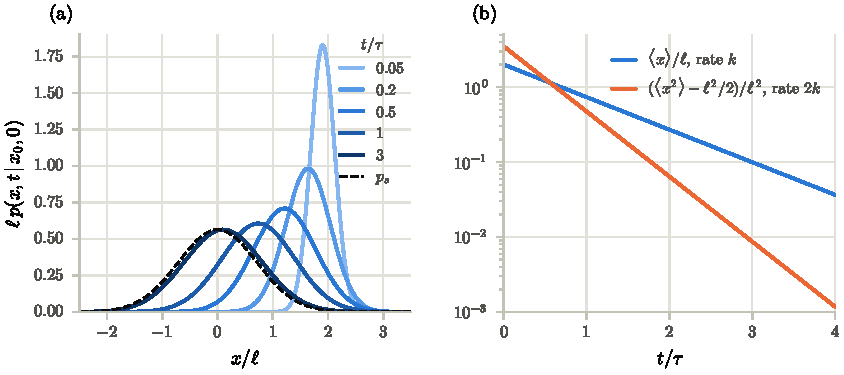
\includegraphics[width=0.9\textwidth]{ou_line.pdf}
    \end{center}
    \vspace{-1em}
    \begin{itemize}
        \small
        \item<2-> $A=-kx$, $B=D$: an optical tweezer ($k=\mathcal K/\gamma$, $\ell=\sqrt{D/k}$). Map $y=xe^{kt}$: free diffusion on the clock $\theta=(e^{2kt}-1)/2k$
        \item<3-> (a) Gaussian, mean $x_0e^{-kt}$, variance $\tfrac12\ell^2(1-e^{-2kt})$; $Q_n\propto H_n(x/\ell)$, $\lambda_n=nk$
        \item<4-> (b) Symmetry selects: $\langle x\rangle$ relaxes at $k$, but $\langle x^2\rangle$ at $2k$
    \end{itemize}
\end{frame}

% =========================================================
% Backup slides (not counted in the footer total)
% =========================================================
\appendix

\begin{frame}{Backup Slides}
    \alert{More examples}
    \begin{itemize}
        \item Free diffusion on the line
        \item Walls by images
        \item Free diffusion on a ring
        \item Constant drift on the half-line
        \item Escape from a harmonic trap
    \end{itemize}
\end{frame}

\begin{frame}{Example: Free Diffusion on the Line}
    \alert{The root of the tree}
    \begin{itemize}
        \item<2-> $A=0$, $B=D$: a colloid in a bulk fluid
        \[ p(x,t\gv x_0,0) = g(x-x_0,t),\qquad g(y,t)=\frac{1}{\sqrt{2\pi Dt}}\,e^{-y^2/2Dt} \]
        \item<3-> Modes $e^{ikx}$, $\lambda=\tfrac12Dk^2$: a continuum down to $0$
        \begin{itemize}
            \item<4-> No gap and no stationary state: algebraic decay, $p(x_0,t)\propto t^{-1/2}$
        \end{itemize}
        \item<5-> Translations: $p$ depends only on $x-x_0$
        \item<6-> Scaling: $p$ is $(Dt)^{-1/2}$ times a function of $(x-x_0)/\sqrt{Dt}$
        \item<7-> Everything below is built from $g$
    \end{itemize}
\end{frame}

\begin{frame}{Example: Walls by Images}
    \demolinks{page=free-summary}{}
    \begin{center}
        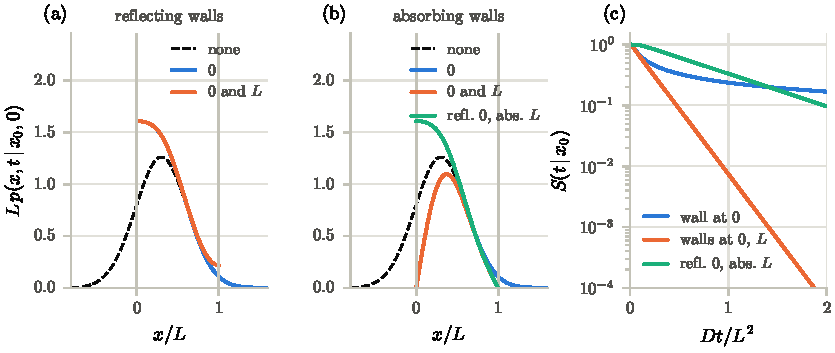
\includegraphics[width=0.92\textwidth]{free_summary.pdf}
    \end{center}
    \vspace{-1em}
    \begin{itemize}
        \small
        \item<2-> Wall at $0$: add a mirror image at $-x_0$, $g(x-x_0)\pm g(x+x_0)$; $+$ is even ($J=0$), $-$ is odd ($p=0$)
        \item<3-> Absorbing half-line: $S=\operatorname{erf}(x_0/\sqrt{2Dt})\sim t^{-1/2}$. Exit is certain, but $\langle T\rangle=\infty$
        \item<4-> Two walls: images of images, an infinite sum $\iff$ the $\cos$ (reflecting) or $\sin$ (absorbing) modes
    \end{itemize}
\end{frame}

\begin{frame}{Example: Free Diffusion on a Ring}
    \demolinks{page=circle}{a=0&b=sqrt(D)&p=D:1&lo=0&hi=1&bc=periodic,periodic&x0=0.5&T=0.2}
    \begin{center}
        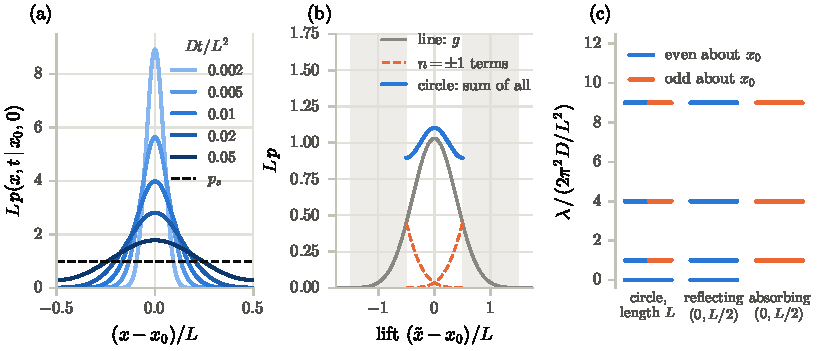
\includegraphics[width=0.92\textwidth]{circle.pdf}
    \end{center}
    \vspace{-1em}
    \begin{itemize}
        \small
        \item<2-> (a) Relaxes to $p_s=1/L$; modes $e^{\pm iq_mx}$, $\lambda_m=\tfrac12Dq_m^2$, $q_m=2\pi m/L$
        \item<3-> (b) The cover: the line's Gaussian plus all its translates by multiples of $L$
        \item<4-> (c) Folding about $x_0$: even modes are the reflecting interval $(0,L/2)$, odd ones the absorbing interval
    \end{itemize}
\end{frame}

\begin{frame}{Example: Constant Drift on the Half-Line}
    \demolinks{page=drift-hl-reflecting}{a=v&b=sqrt(D)&p=v:-1,D:1&lo=0&hi=8&bc=reflecting,open&x0=1&T=10}
    \begin{center}
        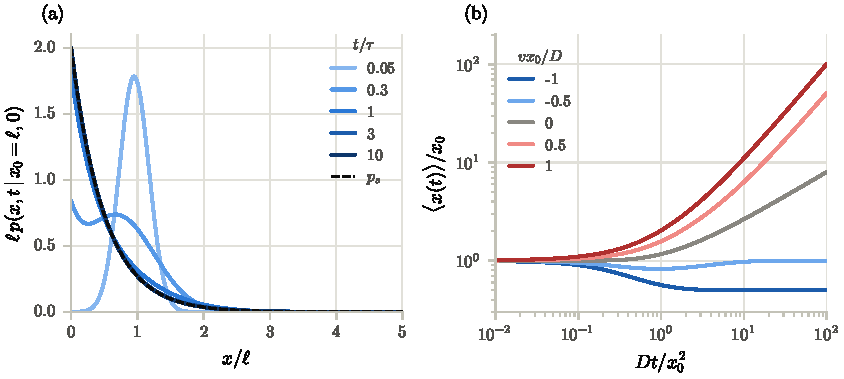
\includegraphics[width=0.9\textwidth]{drift_halfline_reflecting.pdf}
    \end{center}
    \vspace{-1.5em}
    \begin{itemize}
        \small
        \item<2-> $A=v$: sedimentation, an ion in a field. Gauge: $p=e^{\alpha(x-x_0)-t/2\tau}\,u$, $\alpha=v/D$, $\tau=D/v^2$, $u$ free
        \item<3-> Rates are those of $u$ plus $1/2\tau$. Absorbing walls stay absorbing; reflecting ones become Robin, $u'=\alpha u$
        \item<4-> (a) Floor with $v<0$: barometric $p_s\propto e^{-2|v|x/D}$; spectrum $\{0\}\cup[1/2\tau,\infty)$. (b) $\langle x(t)\rangle$
    \end{itemize}
\end{frame}

\begin{frame}{Example: Escape from a Trap}
    \demolinks{page=ou-mixed}{a=-k*x&b=sqrt(D)&p=k:1,D:1&lo=0&hi=2.5&bc=reflecting,absorbing&x0=0&T=50&cond=1}
    \begin{center}
        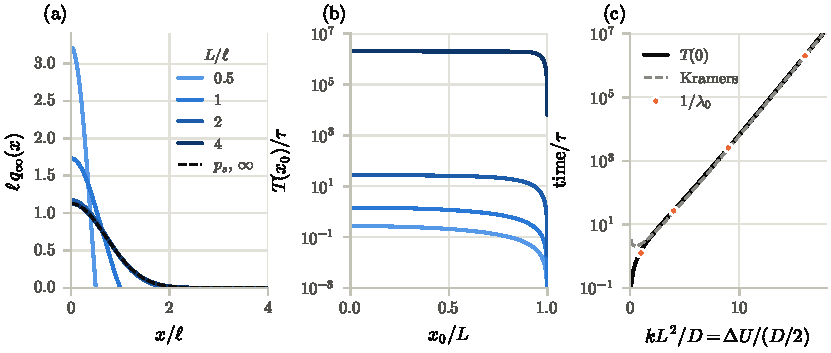
\includegraphics[width=0.9\textwidth]{ou_mixed.pdf}
    \end{center}
    \vspace{-1em}
    \begin{itemize}
        \small
        \item<2-> OU, reflecting at $0$, absorbing at $L$. The map moves this wall: Kummer functions, no further reduction
        \item<3-> (a) QSD $\to$ half-Gaussian: equilibrated in the well. (b) $T(x_0)$ is flat except near the exit
        \item<4-> (c) $\lambda_0\simeq1/T\simeq\frac{2k}{\sqrt\pi}\frac{L}{\ell}\,e^{-L^2/\ell^2}$ (Kramers); the next level is $\sim2k$: metastability
    \end{itemize}
\end{frame}

\end{document}
